% !TEX root = ../../ctfp-print.tex

\lettrine[lhang=0.17]{A}{category} is an embarrassingly simple concept.
A category consists of \newterm{objects} and \newterm{arrows} that go between them. That's
why categories are so easy to represent pictorially. An object can be
drawn as a circle or a point, and an arrow\ldots{} is an arrow. (Just
for variety, I will occasionally draw objects as piggies and arrows as
fireworks.) But the essence of a category is \emph{composition}. Or, if you
prefer, the essence of composition is a category. Arrows compose, so
if you have an arrow from object $A$ to object $B$, and another arrow from
object $B$ to object $C$, then there must be an arrow --- their composition
--- that goes from $A$ to $C$.

\begin{figure}
\centering
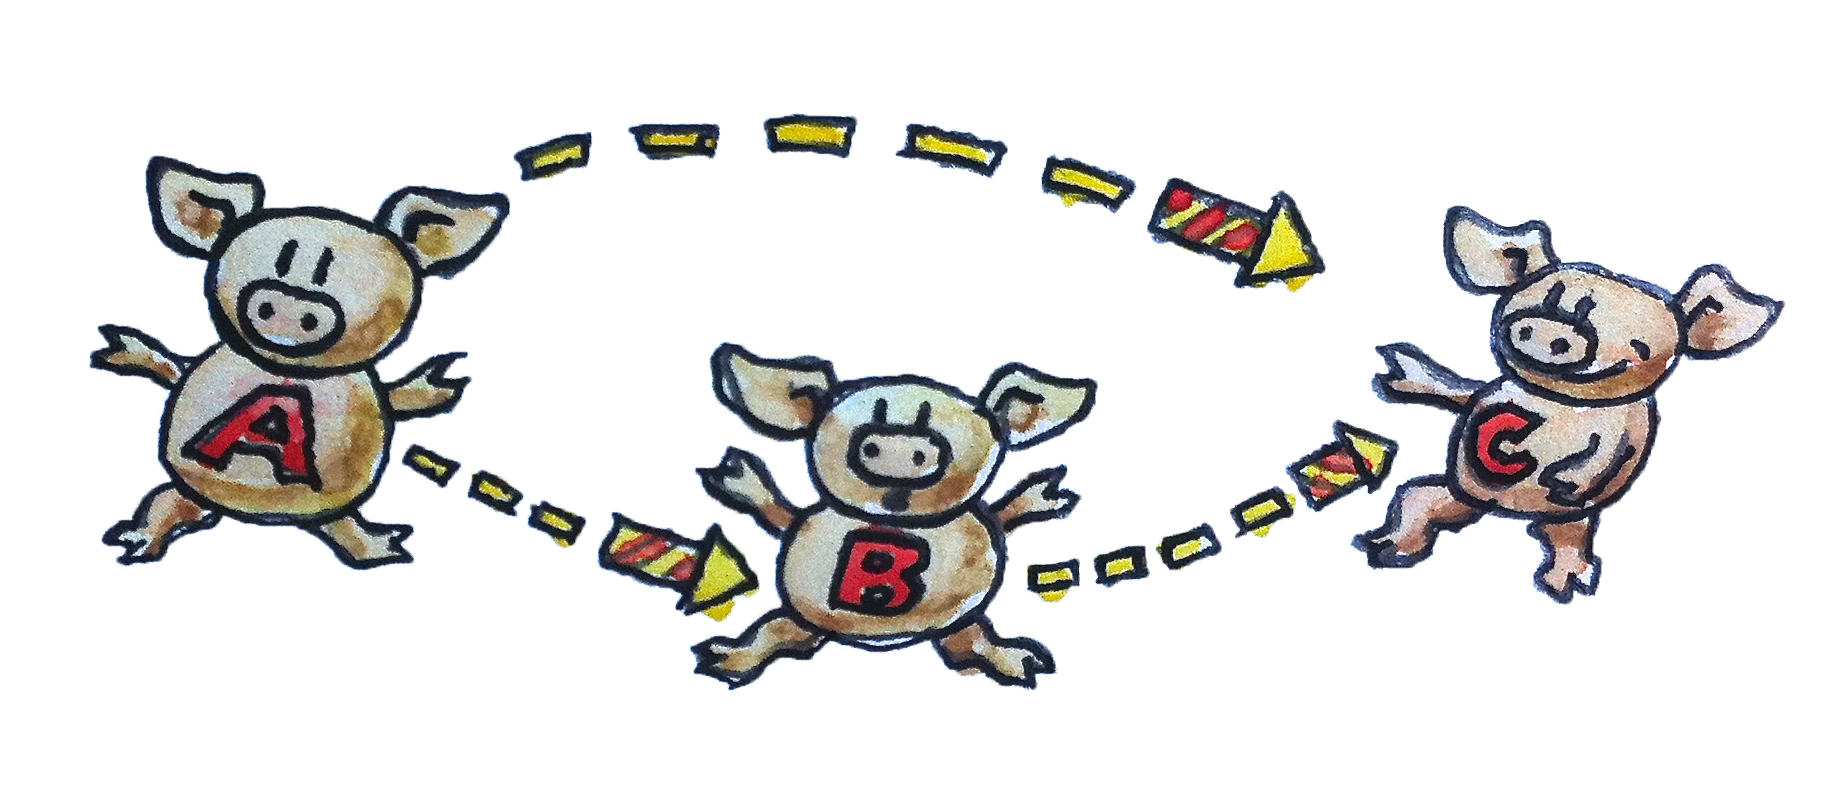
\includegraphics[width=0.8\textwidth]{images/img_1330.jpg}
\caption{In a category, if there is an arrow going from $A$ to $B$ and an arrow going from $B$ to $C$
then there must also be a direct arrow from $A$ to $C$ that is their composition. This diagram is not a full
category because it’s missing identity morphisms (see later).}
\end{figure}

\section{Arrows as Functions}

Is this already too much abstract nonsense? Do not despair. Let's talk
concretes. Think of arrows, which are also called \newterm{morphisms}, as
functions. You have a function $f$ that takes an argument of type $A$ and
returns a $B$. You have another function $g$ that takes a $B$ and returns a $C$.
You can compose them by passing the result of $f$ to $g$. You have just
defined a new function that takes an $A$ and returns a $C$.

In math, such composition is denoted by a small circle between
functions: $g \circ f$. Notice the right to left order of composition. For some
people this is confusing. You may be familiar with the pipe notation in
Unix, as in:

\begin{snip}{text}
lsof | grep Chrome
\end{snip}
or the chevron \code{>>} in F\#, which both
go from left to right. But in mathematics and in Haskell functions
compose right to left. It helps if you read $g \circ f$ as ``g \emph{after} f.''

Let's make this even more explicit by writing some C code. We have one
function \code{f} that takes an argument of type \code{A} and
returns a value of type \code{B}:

\begin{snip}{text}
B f(A a);
\end{snip}
and another:

\begin{snip}{text}
C g(B b);
\end{snip}
Their composition is:

\begin{snip}{text}
C g_after_f(A a)
{
    return g(f(a));
}
\end{snip}
Here, again, you see right-to-left composition: \code{g(f(a))}; this
time in C.

I wish I could tell you that there is a template in the C++ Standard
Library that takes two functions and returns their composition, but
there isn't one. So let's try some Haskell for a change. Here's the
declaration of a function from A to B:

\src{snippet01}
Similarly:

\src{snippet02}
Their composition is:

\src{snippet03}
Once you see how simple things are in Haskell, the inability to express
straightforward functional concepts in C++ is a little embarrassing. In
fact, Haskell will let you use Unicode characters so you can write
composition as:
% don't 'mathify' this block
\begin{snip}{text}
g ◦ f
\end{snip}

You can even use Unicode double colons and arrows:
% don't 'mathify' this block
\begin{snipv}
f \ensuremath{\Colon} A → B
\end{snipv}
So here's the first Haskell lesson: Double colon means ``has the type
of\ldots{}'' A function type is created by inserting an arrow between
two types. You compose two functions by inserting a period between them
(or a Unicode circle).

\section{Properties of Composition}

There are two extremely important properties that the composition in any
category must satisfy.

\begin{enumerate}
\item
Composition is associative. If you have three morphisms, $f$, $g$, and $h$,
that can be composed (that is, their objects match end-to-end), you
don't need parentheses to compose them. In math notation this is
expressed as:
\[h \circ (g \circ f) = (h \circ g) \circ f = h \circ g \circ f\]
In (pseudo) Haskell:

\src{snippet04}[b]
(I said ``pseudo,'' because equality is not defined for functions.)

Associativity is pretty obvious when dealing with functions, but it may
be not as obvious in other categories.

\item
For every object $A$ there is an arrow which is a unit of composition.
This arrow loops from the object to itself. Being a unit of composition
means that, when composed with any arrow that either starts at $A$ or ends
at $A$, respectively, it gives back the same arrow. The unit arrow for
object A is called $\idarrow[A]$ (\newterm{identity} on $A$). In math
notation, if $f$ goes from $A$ to $B$ then
\[f \circ \idarrow[A] = f\]
and
\[\idarrow[B] \circ f = f\]
\end{enumerate}
When dealing with functions, the identity arrow is implemented as the
identity function that just returns back its argument. The
implementation is the same for every type, which means this function is
universally polymorphic. In C++ we could define it as a template:

\begin{snip}{cpp}
template<class T> T id(T x) { return x; }
\end{snip}
Of course, in C++ nothing is that simple, because you have to take into
account not only what you're passing but also how (that is, by value, by
reference, by const reference, by move, and so on).

In Haskell, the identity function is part of the standard library
(called Prelude). Here's its declaration and definition:

\src{snippet05}
As you can see, polymorphic functions in Haskell are a piece of cake. In
the declaration, you just replace the type with a type variable. Here's
the trick: names of concrete types always start with a capital letter,
names of type variables start with a lowercase letter. So here
\code{a} stands for all types.

Haskell function definitions consist of the name of the function
followed by formal parameters --- here just one, \code{x}. The body of
the function follows the equal sign. This terseness is often shocking to
newcomers but you will quickly see that it makes perfect sense. Function
definition and function call are the bread and butter of functional
programming so their syntax is reduced to the bare minimum. Not only are
there no parentheses around the argument list but there are no commas
between arguments (you'll see that later, when we define functions of
multiple arguments).

The body of a function is always an expression --- there are no
statements in functions. The result of a function is this expression ---
here, just \code{x}.

This concludes our second Haskell lesson.

The identity conditions can be written (again, in pseudo-Haskell) as:

\src{snippet06}
You might be asking yourself the question: Why would anyone bother with
the identity function --- a function that does nothing? Then again, why
do we bother with the number zero? Zero is a symbol for nothing. Ancient
Romans had a number system without a zero and they were able to build
excellent roads and aqueducts, some of which survive to this day.

Neutral values like zero or $\id$ are extremely useful when
working with symbolic variables. That's why Romans were not very good at
algebra, whereas the Arabs and the Persians, who were familiar with the
concept of zero, were. So the identity function becomes very handy as an
argument to, or a return from, a higher-order function. Higher order
functions are what make symbolic manipulation of functions possible.
They are the algebra of functions.

To summarize: A category consists of objects and arrows (morphisms).
Arrows can be composed, and the composition is associative. Every object
has an identity arrow that serves as a unit under composition.

\section{Composition is the Essence of Programming}

Functional programmers have a peculiar way of approaching problems. They
start by asking very Zen-like questions. For instance, when designing an
interactive program, they would ask: What is interaction? When
implementing Conway's Game of Life, they would probably ponder about the
meaning of life. In this spirit, I'm going to ask: What is programming?
At the most basic level, programming is about telling the computer what
to do. ``Take the contents of memory address x and add it to the
contents of the register EAX.'' But even when we program in assembly,
the instructions we give the computer are an expression of something
more meaningful. We are solving a non-trivial problem (if it were
trivial, we wouldn't need the help of the computer). And how do we solve
problems? We decompose bigger problems into smaller problems. If the
smaller problems are still too big, we decompose them further, and so
on. Finally, we write code that solves all the small problems. And then
comes the essence of programming: we compose those pieces of code to
create solutions to larger problems. Decomposition wouldn't make sense
if we weren't able to put the pieces back together.

This process of hierarchical decomposition and recomposition is not
imposed on us by computers. It reflects the limitations of the human
mind. Our brains can only deal with a small number of concepts at a
time. One of the most cited papers in psychology,
\urlref{http://en.wikipedia.org/wiki/The_Magical_Number_Seven,_Plus_or_Minus_Two}{The
Magical Number Seven, Plus or Minus Two}, postulated that we can only
keep $7 \pm 2$ ``chunks'' of information in our minds. The details of our
understanding of the human short-term memory might be changing, but we
know for sure that it's limited. The bottom line is that we are unable
to deal with the soup of objects or the spaghetti of code. We need
structure not because well-structured programs are pleasant to look at,
but because otherwise our brains can't process them efficiently. We
often describe some piece of code as elegant or beautiful, but what we
really mean is that it's easy to process by our limited human minds.
Elegant code creates chunks that are just the right size and come in
just the right number for our mental digestive system to assimilate
them.

So what are the right chunks for the composition of programs? Their
surface area has to increase slower than their volume. (I like this
analogy because of the intuition that the surface area of a geometric
object grows with the square of its size --- slower than the volume,
which grows with the cube of its size.) The surface area is the
information we need in order to compose chunks. The volume is the
information we need in order to implement them. The idea is that, once a
chunk is implemented, we can forget about the details of its
implementation and concentrate on how it interacts with other chunks. In
object-oriented programming, the surface is the class declaration of the
object, or its abstract interface. In functional programming, it's the
declaration of a function. (I'm simplifying things a bit, but that's the
gist of it.)

Category theory is extreme in the sense that it actively discourages us
from looking inside the objects. An object in category theory is an
abstract nebulous entity. All you can ever know about it is how it
relates to other objects --- how it connects with them using arrows. This
is how internet search engines rank web sites by analyzing incoming and
outgoing links (except when they cheat). In object-oriented programming,
an idealized object is only visible through its abstract interface (pure
surface, no volume), with methods playing the role of arrows. The moment
you have to dig into the implementation of the object in order to
understand how to compose it with other objects, you've lost the
advantages of your programming paradigm.

\section{Challenges}

\begin{enumerate}
\tightlist
\item
  Implement, as best as you can, the identity function in your favorite
  language (or the second favorite, if your favorite language happens to
  be Haskell).
\item
  Implement the composition function in your favorite language. It takes
  two functions as arguments and returns a function that is their
  composition.
\item
  Write a program that tries to test that your composition function
  respects identity.
\item
  Is the world-wide web a category in any sense? Are links morphisms?
\item
  Is Facebook a category, with people as objects and friendships as
  morphisms?
\item
  When is a directed graph a category?
\end{enumerate}
